\chapter{Situação atual}
Com o aumento da capacidade de passageiros e carga e a 
necessidade de uma maior 
segurança, começou a se fazer necessário trazer ao cockpit vários
documentos como checklist de procedimentos; log book; cartas de 
nevagação, de saída, de aproximação, do aerodromo; tabelas de 
performance da aeronave etc. 

Para levar tudo isto costumava-se usar uma maleta (a Flight Bag),
obviamente esta ficava muito pesada.

Com a minituarização dos computadores e surgimentos os tablets, 
comecaram a ser desenvolvidos programas que subsituiam partes
ou todos estes documentos, é a chamada maleta de voo eletrônica,
mais conhecida pela sigla em Inglês EFB (Electronic Flight Bag).

Nos simuladores de voo para computador pessoal, algumas aeronaves
simulam este equipamento como o Airbus A320neo desenvolvido pela
FlyByWire Simulations. Apesar de ser uma aeronave freeware, ela 
é bem sofisticada chegando ao nível de realismo da Fenix Simulations
ou da ToLiss Simulations, duas produtoras com modelos pagos do A320.

\begin{figure}[ht]
    \begin{center}
    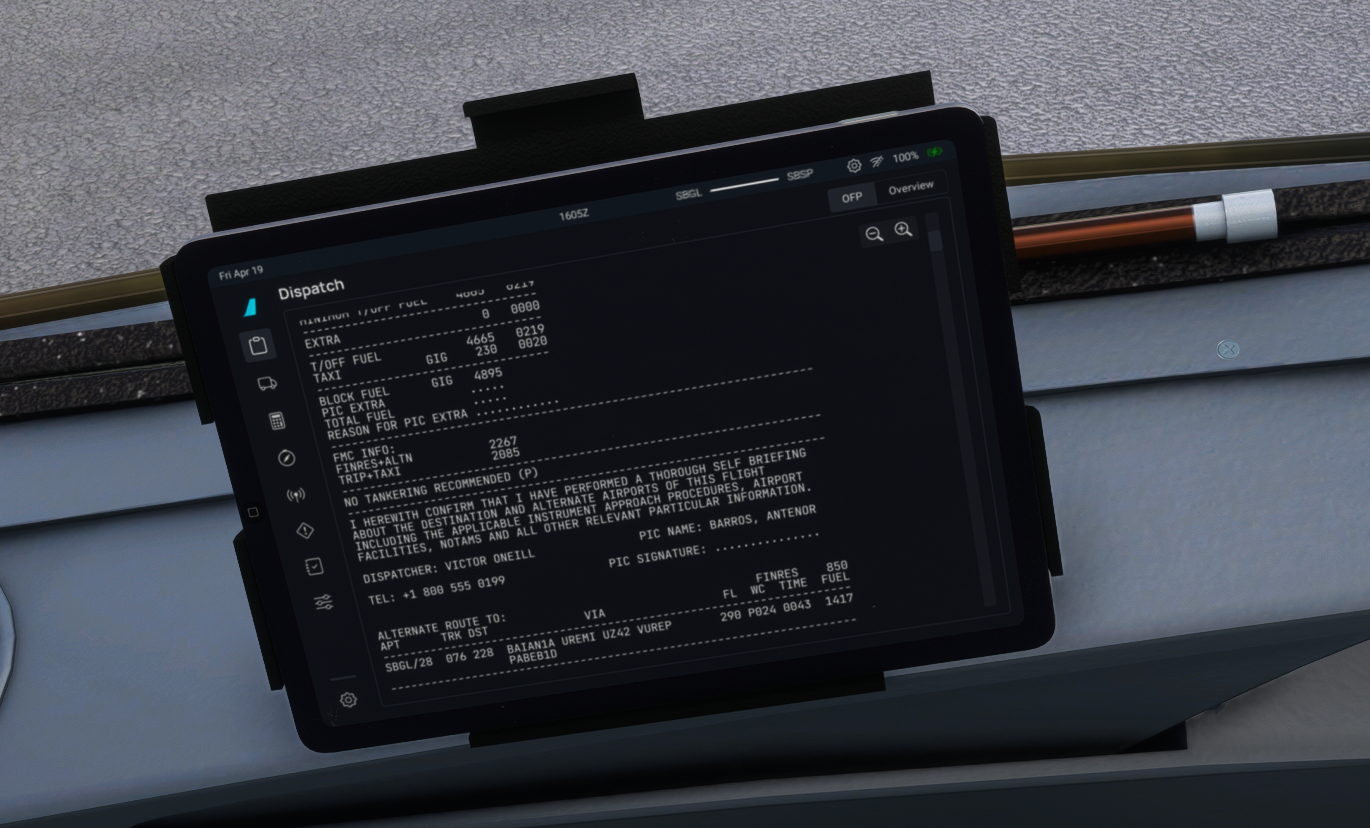
\includegraphics[width=400pt]{img/efb-a320.png}
    \caption{Exemplo de um EFB no Flight Simulator 2020 na aeronave A320neo}
    \label{fig:efb-a320}
    \end{center}
\end{figure}

Contudo, o METAR do aeródromo não se encontra disponível no EFB.
É possível usar o computador de bordo da aeronave (FMC) e conseguir
esta informação. Também é possível sintonizar na frequência do ATIS,
mas isto só funcionará se o avião já estiver perto de aeródromo.

O que muitos jogadores fazem é acessar o AISWEB, sistema oficial brasileiro
de informações aeronáuticas. 

\begin{figure}[ht]
    \begin{center}
    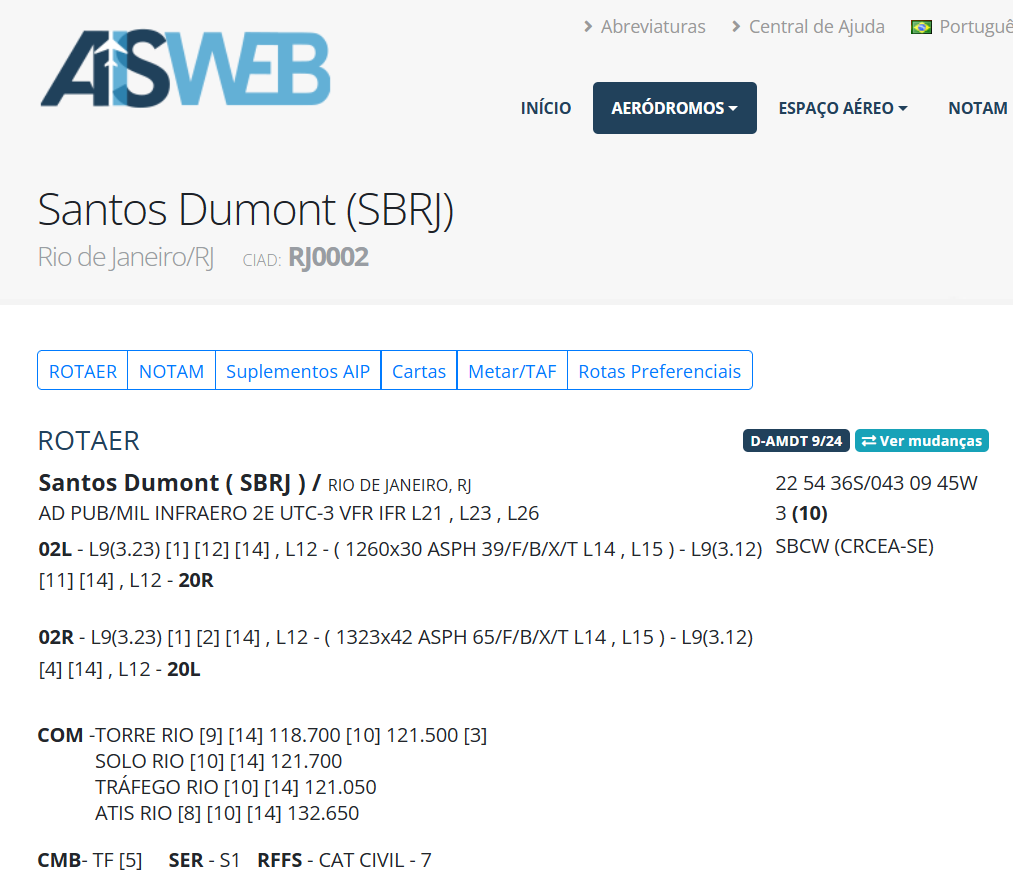
\includegraphics[width=400pt]{img/aisweb.png}
    \caption{AISWEB com informações de pista frequências de comunicação e navegação para o Santos Dumont}
    \label{fig:aisweb}
    \end{center}
\end{figure}

É um site extremamente completo, podendo
ser usado em operações reais, mas para o jogador iniciante seria 
de valia uma interface mais simples.